\documentclass[./chapitre3.tex]{subfiles}
\begin{document}

\section{Core Module}
The core module is the base module of the library. It contains the core classes and functions
that are used by the other modules. It is crucial that the core module is well designed and
focus on stability, performance and extensibility. From the requirement specifications we can
identify that the file\_io, network\_io and processing modules will need to use a \lstinline|Frame| and a
\lstinline|Cluster| class. The \lstinline|Frame| class will contain the data sent by the detector and the \lstinline|Cluster| class
will contain the data after processing. Hence the core module will define these two classes/interfaces.\\

\subsection{Class Diagram}
Figure \ref{fig:core_class_diagram} shows the class diagram of the core module. The attributes
and methods of the classes are not shown in the diagram for simplicity.

\begin{figure}
    \centering
    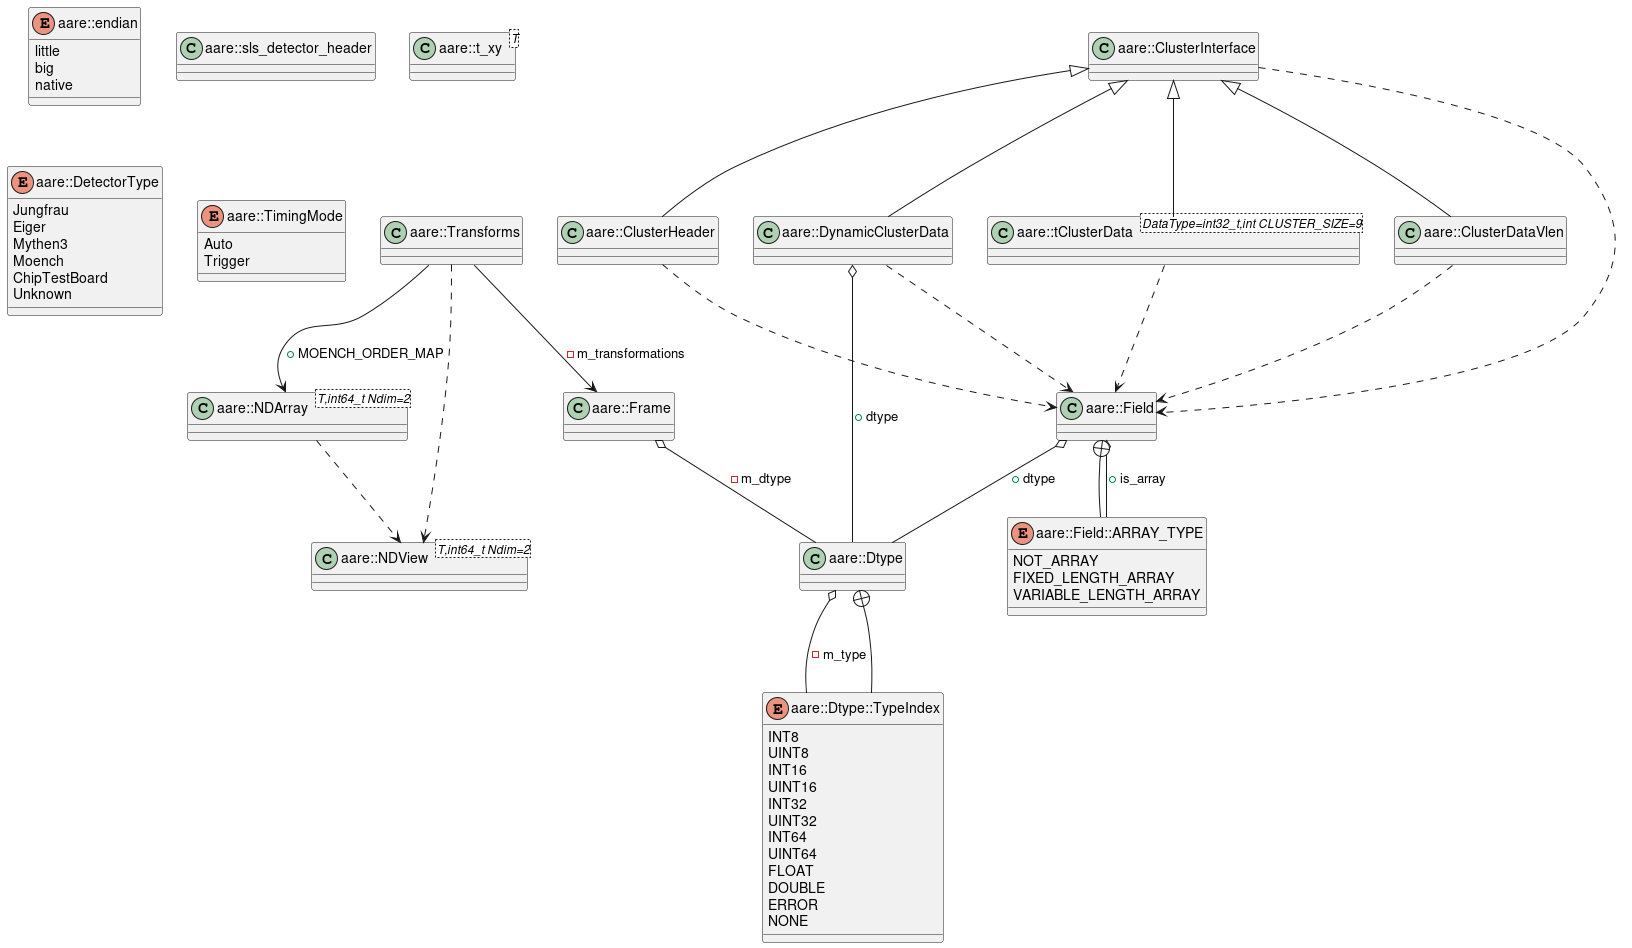
\includegraphics[width=\textwidth]{Chapitre3/figures/core_class_simplified.png}
    \caption{Core module simplified class diagram}
    \label{fig:core_class_diagram}
\end{figure}
\subsection{Dtype Class}
The library will need to read write data from multiple streams such as files, network, memory...
The library will also handle different data types such as integers, floats... The Dtype class
is used to represent the data type of the handeled stream of bytes. The Dtype class also
define the endianness of the data. To represent the data types, this class internally uses an enum
class. String representation can also be used to create a Dtype object. The string representation
is defined as "\textless" or \textgreater" for little or big endian followed by the data type and its size in bytes.
For example "\textless i4" represents a little endian int32 and "\textgreater f8" represents a big endian float64.
\\

The Dtype class is also very important for transferring data between the C++ and Python bindings.
The Python bindings will use the Numpy library to handle the data. Numpy uses the python standard
of buffer protocol\cite{bufferprotocol} to handle data exchange. The buffer protocol is a way to expose the data of an object
to other objects. It is useful when we don't want to copy the data but just share it.
The library allows data to go from C++ to Python and vice versa with or without copying.
The Dtype class is used to define the data type of the incoming of outgoing buffer.\\

\subsection{Frame Class}
The \lstinline|Frame| class contains the data of a detector "image". The data is stored in a buffer of bytes.
and it uses Dtype to define the data type of the buffer. The \lstinline|Frame| class also contains the shape
of the data.\\

\lstinline|Frame| objects will be used across the library. The file\_io module will use \lstinline|Frame| objects to read
and write data from files. The network\_io module will use \lstinline|Frame| objects to send and receive data
over the network. The processing module will use \lstinline|Frame| objects to process its data. Therefore
it is very important that the \lstinline|Frame| class is as simple as possible and as general as possible
to be used by all the modules.\\

In the first iterations of the library, the \lstinline|Frame| class was templated on the type of the data.
This allowed the user to manipulate the data of the frame directly e.g. \lstinline[language=C++]|Frame<int32_t>[x][y] = value| .
However, this is now considered a bad design choice. Templating \lstinline|Frame| forced the user to know the type
of the data before creating a \lstinline|Frame| object. It also propoagated complexity to higher level
layers. For example, file\_io functions that read data from a file and returned
Frame objects also had to be templated and so on. This is why the \lstinline|Frame| class is now a simple class untemplated
on the data type. and this point is why NDView and NDArray were introduced.

\subsection{NDView and NDArray}
The NDView and NDArray classes are used to manipulate the data of a Frame object or other buffers. They stand for
N-Dimensional View and N-Dimensional Array. The NDView class is a non-owning view of the data. It is used to access
the data of a buffer without copying it. It can also be used to reshape (in numpy terms) the data. NDArray is an
owning view of the data. It copies the data of the buffer and owns it.\\

The NDView and NDArray classes are very helpful for processing the data. They are inspired by the Numpy library
which is a powerful library for numerical computing in Python \cite{harris2020array}. The Numpy library had a huge
influence on the development of python libraries and it is widely used accross different fields.
Users of this library can reuse their knowledge of Numpy and apply it to this library. This helps
to reduce the learning curve of the library and accelerates its adoption.
In addition, When the library receives a numpy object from python it can be converted to a NDView/NDArray object and vice versa. \\

\subsection{Cluster Classes}
We refer to the group of classes that handle cluster data the Cluster classes. The Cluster classes have gone through multiple iterations.
From working around the limits C++ and Python bindings to
balancing the tradeoffs of performance vs flexibility vs ease of use. This has led us to the current design of the Cluster classes.\\

After receiving frames from disk or the network a common way to process the data is to find the photon of electron clusters in
the image. A cluster is a group of pixels that are close to each other and have a high intensity. The cluster finding algorithm
will be part of the processing module and is beyond the scope of the core module. Clusters need to be generated, saved and read from
files and in future iterations sent over the network. This is why a unified Cluster class definition is needed in the core module.\\

Clusters are represented as a list of pixels. There's no single way to represent a cluster. The group currently uses multiple
forms of clusters such as: fixed length clusters which are a list of pixels of a fixed size (3x3 or 2x2) centered around the maximum pixel.
and variable length clusters which are a list of pixels that are adjacent to each other. Different cluster formats have different uses and
applications. For example fixed size clusters are more commonly used for photon clusters while variable size clusters are more commonly used
electron clusters as they leave a trail of pixels.\\

Given these requirements, First an interface class was created to set the define the methods that a Cluster class should have.
This interface class is only used to inherit its methods in case the subsclass does not implement them. It should be
noted that the interface class does not contain any virtual methods and is not meant to be used as a polymorphic
class. Any implementation of a Cluster class should inherit from the ClusterInterface class. Although it isn't
implemented, the ClusterInterface can use the Curiously Recurring Template Pattern (CRTP) and Substitution failure
is not an error (SFINAE) idioms to enforce that the subclass implements the methods in compile time.\\

First we will explain the general design of a Cluster class. The structure of a Cluster object is defined by a
list of Field objects. A Field object is a simple class that contains a label (\lstinline[language=C++]{std::string}), a
dtype (\lstinline[language=C++]{Dtype}) an enum is\_array that defines if the field is a scalar or fixed length array or a
variable length array and finally a size attribute that is used to indicate the size of the fixed length array.

Example \ref{lst:cluster_structure} the definition of the structure of a Cluster object to represent a 3x3 int32 cluster
that also contains an x and a y attributes:
\begin{lstlisting}[language=C++, caption={Example: Definition of a Cluster structure},label={lst:cluster_structure}]
// cluster definition
struct Cluster{
    int32_t x;
    int32_t y;
    int32_t pixels[9];
};

// cluster fields description
std::vector<Field> fields = {
    Field("x", Dtype("<i4"), Field::Scalar),
    Field("y", Dtype("<i4"), Field::Scalar),
    Field("pixels", Dtype("<i4"), Field::FixedLengthArray, 9)
};
    \end{lstlisting}

Given that we can define the structure of a Cluster object, we can define a DynamicCluster class that holdes the data of any
cluster and interprets it according to the structure. The DynamicCluster offers set and get methods to manipulate and access
its data.\\

Although the DynamicCluster class is very flexible and can be used to represent any type of cluster, it is not the most efficient
way to represent all clusters. DynamicCluster allocates its data on the heap and its contents is spread accross the memory.
For fixed size clusters this is not efficient as the data can simply be represented in a struct and be stored in contiguous
memory.

Example \ref{lst:read_clusters} shows how to read multiple clusters from a file directly to memory. This is not possible
with the DynamicCluster class. This is why \lstinline|tCluserData<typename DataType,int CLUSTER_SIZE>| has been introduced.

The tClusterData class is a templated class that represents a fixed size cluster. The data will be stored contiguously in
stack memory. The tClusterData class is more efficient than the DynamicCluster class but it is less flexible.\\
\begin{lstlisting}[language=C++, caption={Example: Reading multiple clusters from a file},label={lst:read_clusters}]
struct Cluster {
    int32_t x;
    int32_t y;
    int32_t pixels[9];
}; // 3x3 cluster
std::vector<Cluster> clusters(10); // list of 10 clusters stored contiguously in memory
fread(clusters.data(), sizeof(Cluster), clusters.size(), file); // directly read 10 Clusters to memory
    \end{lstlisting}


These were tha main components of the core module. It also includes other classes and enums that are less important
but are used by the other modules.
% Figure \ref{fig:core_class_diagram} shows the full class diagram of the core module.\\

% \begin{figure}
%     \centering
%     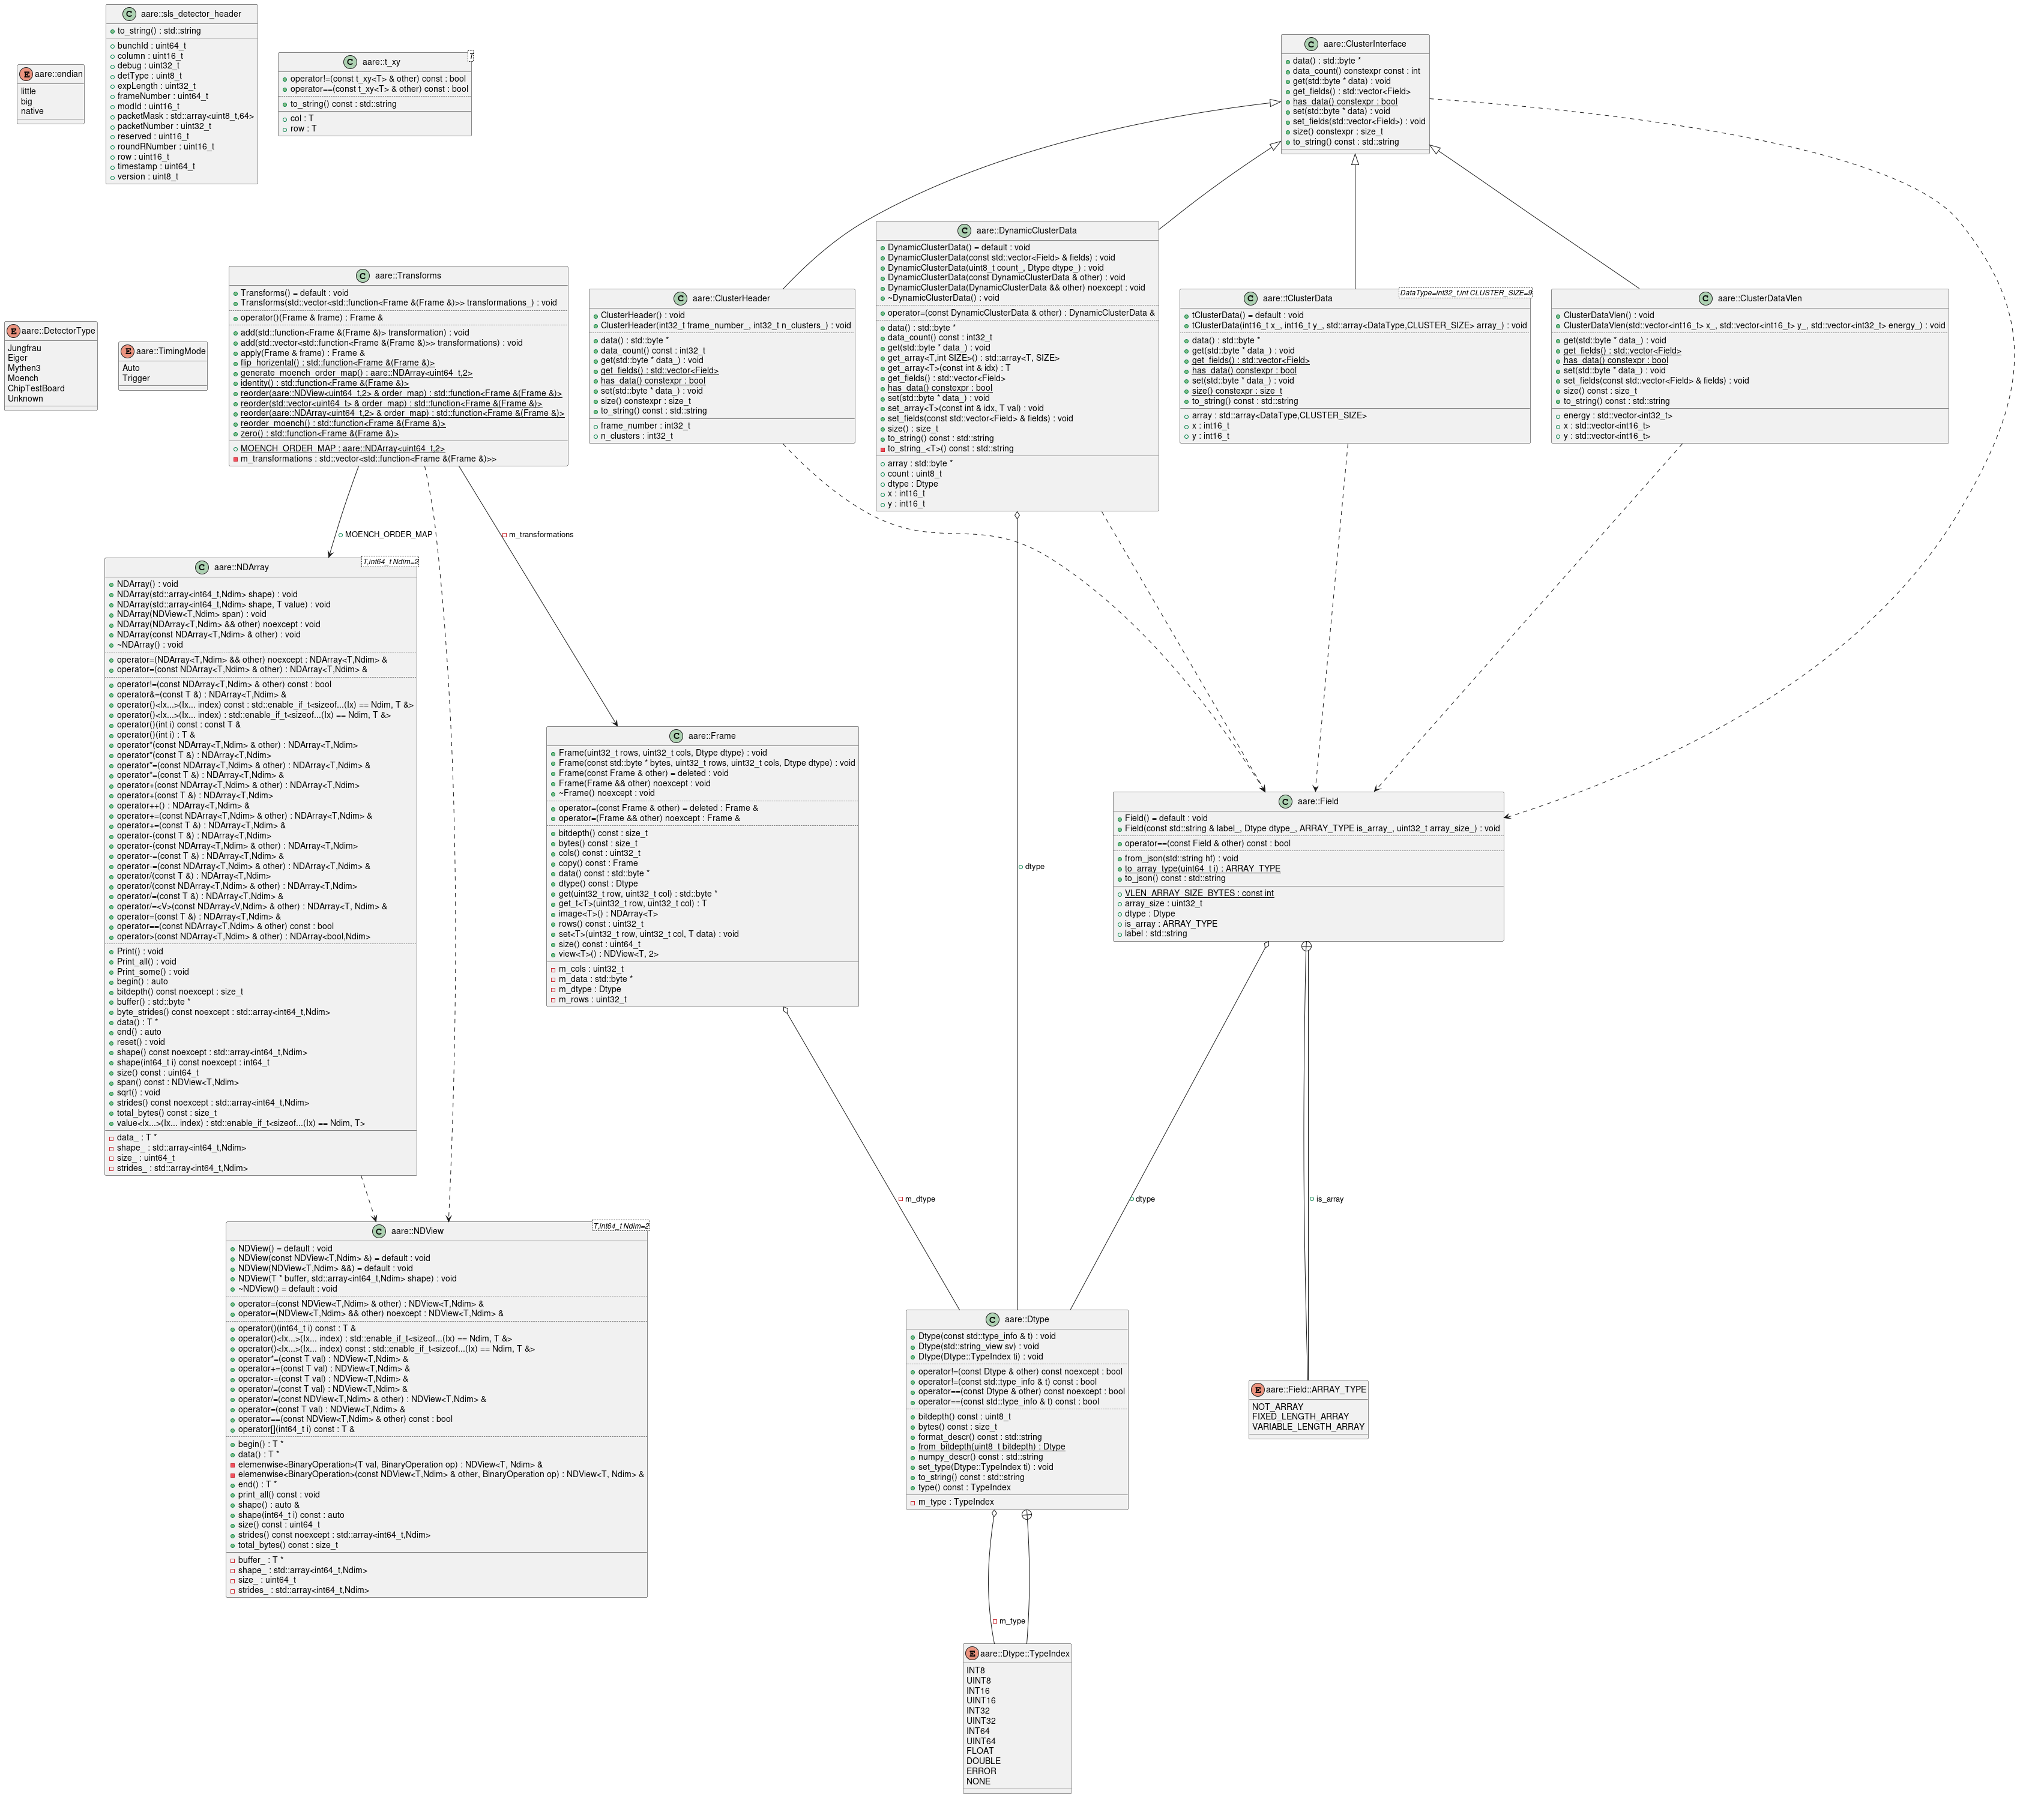
\includegraphics[width=\textwidth]{Chapitre3/figures/core_class.png}
%     \caption{Core module class diagram}
% \end{figure}






\section{File IO Module Implementation}
In this section we will go through the design and implementation of the file\_io module.
The file\_io module is in general responsible for storing data structures and reading them from disk.
Specifically it should offer features to read and write Frame and Cluster objects to the disk.\\

\begin{figure}
    \centering
    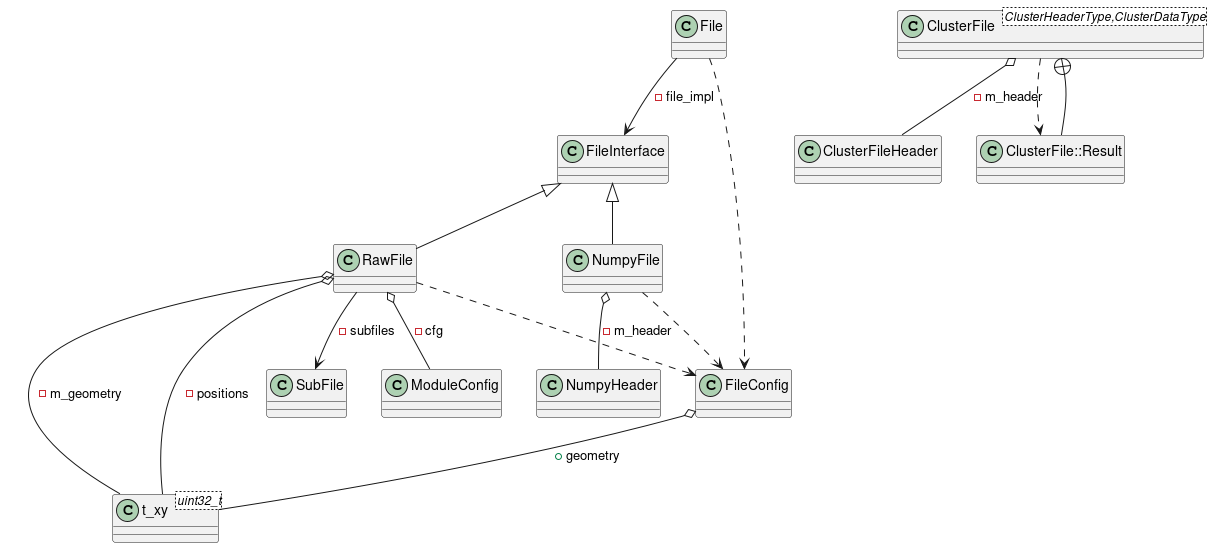
\includegraphics[width=\textwidth]{Chapitre3/figures/file_io_class.png}
    \caption{File IO module class diagram}
    \label{fig:file_io_class}
\end{figure}
Figure \ref{fig:file_io_class} shows the class diagram of the file\_io module.
The module is composed of two parts for handling Cluster  and Frame objects.\\

\subsection{Frame IO}
Reading and writings Frame objects to disk is a central feature of the library. The library
should focus on performance and flexibility when reading and writing Frame objects.
Performance is important as the library should be able to read and write huge amounts of data
quickly. Flexibility is important because different file formats can be used to store the data e.g.
Binary, HDF5, Numpy...\\

From the existing slsDetectorPackage library, frame data is stored in a binary format.
A master file written in JSON contains the metadata of the data and a .raw file contains the data itself.
For compatibility reasons with an old master file format, the library also must handle master files written in text
format following a predefined structure.

In addition, since many users of the library will be using Python, the C++ library should
read and write Numpy files. A Numpy file is composed of a metadata header in plain text and
a binary part that contains the data.\\

As seen in the class diagram \ref{fig:file_io_class}, the \lstinline|FileInterface| class
is the base class for \lstinline|NumpyFile| and \lstinline|RawFile|. \lstinline|FileInterface|
is an abstract class that only has pure virtual methods. A pointer to \lstinline|FileInterface|
can point to either a \lstinline|NumpyFile| or a \lstinline|RawFile| object. This allows the
user to use the same interface to read and write different file formats.

The interface offers functions such similar to the familiar C file API such as \lstinline|read()|
to read a Frame, \lstinline|read(int n)| to read n Frames, \lstinline|seek(int n)| to move the
file pointer to the n-th Frame, \lstinline|write(Frame& frame)| to write a Frame.\\

To use C++'s inheritance and polymorphism features, pointers to the base class are used
(e.g. \lstinline|FileInterface* file = new NumpyFile()|). However, forcing the user to use
pointers is not very user-friendly and can lead to memory leaks. This is why a \lstinline|File|
class following RAII idiom is introduced. It is a simple class that contains a pointer to
the base class and manages the memory of the pointer. The user can use the \lstinline|File|
class to read and write files without worrying about memory management.\\

Furthermore, to optimize the reading and writing of \lstinline|Frame| objects, the
library implements the appropriate copy and move constructors and assignment operators.
This avoids unnecessary copying of the data and improves the performance of the library.\\

\begin{lstlisting}[language=C++, caption={Example: Reading and writing a Frame from a file},label={lst:read_frame}]
// reading a Frame from a file
File file1("data.npy");
Frame frame = file.read();

// writing a Frame to a file
auto dtype = Dtype("<u4"); // unsigned int32
FileConfig const config = {dtype, 100, 100}; // File holds 100x100 Frames of uint32_t
File file2(path, "w", config); // open file in write mode
file2.write(frame); // write the frame to the file
// file is closed when it goes out of scope
\end{lstlisting}

Example \ref{lst:read_frame} shows how to read and write a Frame from a file. The \lstinline|File|
recognizes the file format from the extension of the file and creates the appropriate object.
Here in this example, a \lstinline|NumpyFile| object will be constructed.
Following RAII idiom, the file is closed and memory is freed when the \lstinline|File|
object goes out of scope. As seen from this example the \lstinline|File| abstracts a lot
of the complexity of reading and writing files.\\

\subsection{Cluster IO}
The Cluster IO part of the file\_io module is responsible for reading and writing Cluster objects to disk.
The Cluster part of the file\_io module went through multiple iterations. The first iteration
handeled fixed size clusters only. This, of course, needed to change after the introduction
of the DynamicCluster class. Currently, the module is implemented to handle fixed size,
variable size and upcoming custom clusters.\\

A new file format has been introduced to store clusters and to unify the storage of different
types of clusters. The file format is composed of a FileHeader written in plain text and a binary
data part that contains the clusters. The header contains the metadata of the file such as
the version, the number of records stored, the structure of the clusters... The header is
written in plain text JSON format to be human-readable.

The binary data part contains the
records. A record is a ClusterHeader followed by N-Clusters. A ClusterHeader contains the
metadata of the record such as the number of clusters, frame number...

The structure of the ClusterHeader and ClusterData are defined in the FileHeader.\\

The library allows users to define their own cluster structures. Whether it is
a custom ClusterHeader or a custom ClusterData, ClusterFile will be able to read and write
it. It is also very important to manage the tradeoffs of this flexibility and performance
requirements. Unlike dynamic languages such as Python or Javascript, C++ is a statically typed
language. This means that the library must know the structure of the clusters at compile time.
Allowing the user to define their own cluster structures can lead to a lot of complexity.
This is why it is important to find a balance between flexibility and performance.\\

Having noted some of the limitations of C++, some of them can be overcome by using templates.
The ClusterFile class is templated on the ClusterHeader and ClusterData types. This allows
the user to define their own ClusterHeader and ClusterData types that follow the ClusterInterface.
The ClusterFile class will be able to read and write these clusters. ClusterFile also
checks if the structure's data are stored contiguously in memory. If they are, the library
can read and write clusters from disk with one system call. This is much faster than reading
and writing clusters one by one.\\

\begin{lstlisting}[language=C++, caption={Example: Reading and writing a Cluster from a file},label={lst:read_cluster}]
// reading a Cluster from a file
ClusterFile<ClusterHeader, ClusterData> file("data.clust2");
auto result = file.read(); // read 1 record from file
ClusterHeader header = result.header;
std::vector<ClusterData> clusters = result.data;

// writing a Cluster to a file
 ClusterFileHeader header;
// define the ClusterHeader fields
header.header_fields.push_back({"frame_number", Dtype::INT32, Field::NOT_ARRAY});
header.header_fields.push_back({"n_clusters", Dtype::INT32, Field::NOT_ARRAY});

// define the ClusterData fields
header.data_fields.push_back({"x", Dtype::INT16, Field::NOT_ARRAY});
header.data_fields.push_back({"y", Dtype::INT16, Field::NOT_ARRAY});
header.data_fields.push_back({"pixels", Dtype::INT32, Field::FIXED_LENGTH_ARRAY, 9});
ClusterFile<ClusterHeader, ClusterData> file("file.clust2", "w", header);

ClusterHeader header = {1, 10}; // 1st frame, 10 clusters
std::vector<ClusterData> clusters = {{1, 2, {1, 2, 3, 4, 5, 6, 7, 8, 9}}};
file.write(header, clusters);
\end{lstlisting}


Although the task of reading and writing user defined data types is complex, the library
abstracts a lot of the complexity. The user only needs to define the structure of the clusters
and the library will take care of the rest. Example \ref{lst:read_cluster} shows how to read
and write custom clusters from a file.\\

A hidden but important disadvantage of the current implementation is that the ClusterFile
class is templated on the ClusterHeader and ClusterData types. In C++, this is not a problem
as long as the ClusterHeader and ClusterData types are known at compile time. However, the python
bindings will need to know the ClusterHeader and ClusterData types at compile time. This prohibits
python users from defining their own cluster structures. Furthermore, the shared object file
that is generated by the C++ library will be much larger. As it will contain all the possible
ClusterHeader and ClusterData types. This is a tradeoff that the library has to make.\\

In conclusion, the ClusterFile class is a very powerful class that allows the user to read
and write customly defined structures from disk. It is also optimized for performance. Stack
based structures are read and written in bulk. Minimizing the number of OS file API calls.
However, the ClusterFile class is templated on the ClusterHeader and ClusterData types. This
can lead to large shared object files and prohibits the python bindings from defining their
own cluster structures.\\


\section{Network IO Module Implementation}
The network\_io module is responsible for sending and receiving Frame objects over the network.
The module should interoperate with the existsing system programs such as the slsReceiver.\\

\begin{figure}
    \centering
    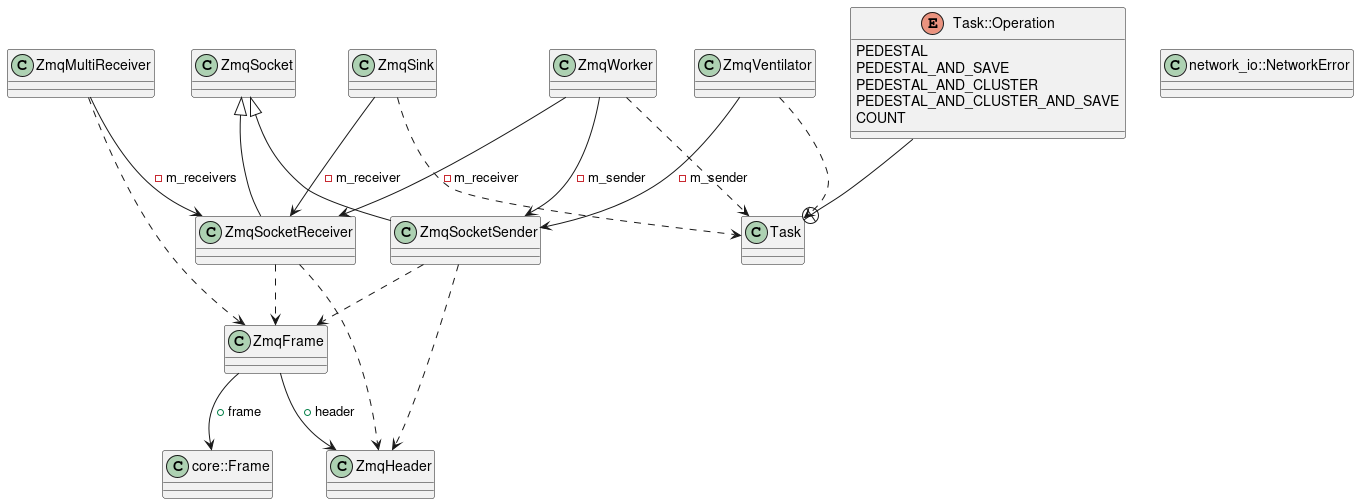
\includegraphics[width=\textwidth]{Chapitre3/figures/network_io_class.png}
    \caption{Network IO module class diagram}
    \label{fig:network_io_class}
\end{figure}

Figure \ref{fig:network_io_class} shows the class diagram of the network\_io module.\\

\subsection{ZeroMQ}
The network\_io module uses ZeroMQ as the network library. ZeroMQ is a high-performance
asynchronous messaging library that provides a message queue, but unlike message-oriented
middleware, a ZeroMQ system can run without a dedicated message broker. ZeroMQ is a very
powerful library that can be used to build complex network systems. It is also very easy
to use and has bindings for many languages. \cite{hintjens2013zeromq} \\

ZeroMQ's model provides socket communication between threads, processes and network nodes.
Its sockets can work with Inter Process Communication (IPC), Transmission Control Protocol (TCP),
User Datagram Protocol (UDP), WebSockets and more. ZeroMQ sockets can be connected with each other
following a plethora of different patters. The most common patterns are Request-Reply,
Publish-Subscribe, Push-Pull, Pair, and Router-Dealer etc.\\

ZeroMQ's philosophy is to provide a simple API that can be used to build complex systems.
It is very flexible and extensible while also being very fast. This aligns with our library's
philosophy of being easy to use, flexible and efficient.\\

\subsection{ZmqSocket classes}
As seen from the class diagram, the network\_io module implements ZmqSocketReceiver and ZmqSocketSender.
These classes are responsible for receiving and sending Frame objects over the network. They
derive from the ZmqSocket class which is a wrapper around the ZeroMQ socket.\\

The ZmqSocket class follows the RAII idiom and wraps around the ZeroMQ socket. The ZmqSocketReceiver
and ZmqSocketSender classes will be used by users to communicate with slsReceiver and
other network nodes.\\

The network\_io module methods return a ZmqFrame object. It is a wrapper around Frame that adds
network metadata to it.\\

\begin{lstlisting}[language=C++, caption=Example of using the network\_io module, label=lst:network_io_example]
ZmqSocketReceiver socket("tcp://localhost:5555"); 
socket.connect(); // connect to another node
std::vector<ZmqFrame> v = socket.receive_n(); // receive frames until a stop signal
ZmqSocketSender socket2("tcp://localhost:5556");
socket2.bind(); // bind to a port
Frame frame(512,512,Dtype::UINT32); // create a Frame object
ZmqHeader header;
header.shape = {512,512}; // set the metadata of the frame
ZmqFrame zmq_frame = {header, frame}; // create a ZmqFrame object
socket2.send(zmq_frame); // send the frame
\end{lstlisting}


Example \ref{lst:network_io_example} shows how to use the network\_io module to send and receive frames.
The RAII idiom as always comes in handy to disconnect sockets, free resources and close connections when the
object goes out of scope.\\


\subsection{ZmqMultiReceiver class}
In several scientific experiments, multiple detectors are used to capture data. Whether
it is to capture data from different angles, different parts of the sample or to balance
the load, multiple detectors are used.\\

\begin{figure}
    \centering
    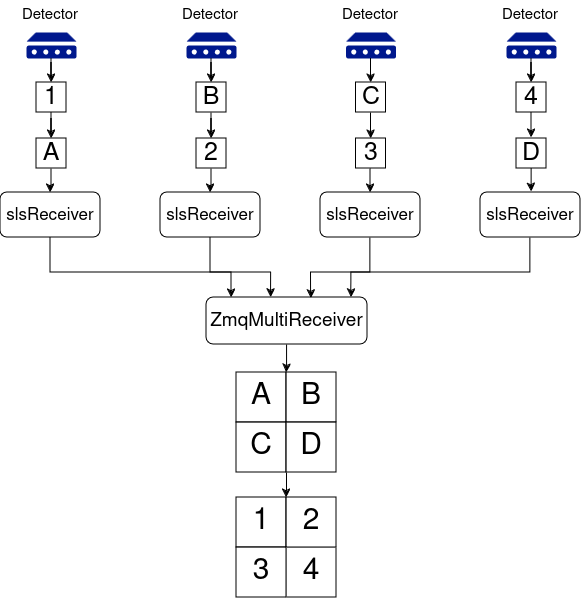
\includegraphics[width=\textwidth]{Chapitre3/figures/zmqmulti.png}
    \caption{Illustration of the ZmqMultiReceiver class: multiple detectors send frames to the ZmqMultiReceiver
        which combines them into a single Frame. The ZmqMultiReceiver also manages the synchronization between streams.}
    \label{fig:zmq_multi_receiver}
\end{figure}

The ZmqMultiReceiver class is a wrapper around multiple ZmqSocketReceiver objects. It is used
to receive data from multiple sources and combine them into a single stream of frames. The user of this class
must specifiy the different endpoints to connect to as well as the geometry to form the frames.\\

The ZmqMultiReceiver handles the synchronization of the different streams. Detectors can drop
frames, send them at different rates or have different delays. The ZmqMultiReceiver class
must account for these issues and provide a consistent stream of frames. Fault tolerance is also
important and adequate error handling and logging must be implemented.\\

Instead using multiple threads to listen to each detector, the ZmqMultiReceiver class uses a single
thread to listen to all the detectors. It uses a poller to listen to all the sockets and receive
frames. ZeroMQ simplifies the polling operation by providing a \lstinline|zmq::poll()|
function that can be used to poll the sockets' file descriptors. On Linux systems,
\lstinline|zmq::poll()| uses the kernel's \lstinline|epoll| interface.

epoll is a Linux kernel system call that waits for events on file descriptors (sockets). It is used for
multiplexing I/O to manage multiple connections. epoll is more efficient than the older select system call
and can handle a large number of connections. Several webserver implementations such as nodejs use epoll to handle
thousands of HTTP requests concurrently. \cite{gammo2004comparing, marathe2015introduction}\\

\subsection{Task Distribution}
The network\_io module offers classes to support task distribtion over the network.
Detectors are extremely fast can reach more than 10GB/s and combining multiples of them
can lead to bottlenecks in network.

In addition, Some experiments
can run for multiple hours and even multiple days. Storing the data on disk will become expensive
overtime. 24 hours with 10GB/s leads to 864TB of data. This is why it is required to
process data in real time and store only the relevant results.

For these reasons distributing the bandwidth and computation to multiple machines
is the way to go.\\

\begin{figure}
    \centering
    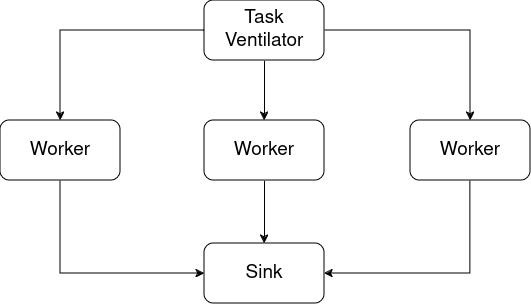
\includegraphics[width=\textwidth]{Chapitre3/figures/task_distribution.png}
    \caption{Illustration of the task distribution system. The task ventilator class distributes
        tasks to multiple workers. The workers process the tasks and send the results back to the
        sink.}
    \label{fig:task_distribution}
\end{figure}

Figure \ref{fig:task_distribution} illustrates the task distribution system. For example the task
ventilator receives frames from multiple detectors. It then creates a Task object that contains
the data and specifies the steps to manipulate the data (if needed). The task ventilator
distributes the tasks to multiple workers. The workers process the tasks and send the results
back to the sink. The sink is used to collect the results synchronize and store them if needed.\\

The library provides helper classes that wrap around the ZmqSocketSender and ZmqSocketReceiver
to implement the task distribution system. The \lstinline|ZmqVentilator|, \lstinline|ZmqWorker|
and \lstinline|ZmqSink| classes handle the network side of the task distribution system.\\

Workers connect upstream to the ventilator, this means that we can add or
remove workers arbitrarily at runtime. With fair-queuing the sink collects
results from the workers evenly \cite{hintjens2013zeromq}. The current library
does not support using multiple ventilators and sinks.\\

\begin{lstlisting}[language=C++, caption=Example of a task ventilator, label=lst:task_ventilator]
    ZmqSocketReceiver receiver(endpoint);
    receiver.connect();

    // 1. create ZmqVentilator
    ZmqVentilator ventilator("tcp://*:4321");

    // 2. receive frame from slsReceiver
    std::vector<ZmqFrame> zmq_frames = receiver.receive_n();

    for(auto &zmq_frame : zmq_frames){
        // 3. create task
        Task task = Task::init(zmq_frame);
        task.id = zmq_frame.header.frameNumber;

        // 4. push task to ventilator
        ventilator.push(task);
    }
\end{lstlisting}

\begin{lstlisting}[language=C++, caption=Example of a worker, label=lst:task_worker]
    // 1. create ZmqWorker
    ZmqWorker worker(ventilator_endpoint, sink_endpoint);
    worker.connect();

    while(true){
        // 2. receive task from ventilator
        Task task = worker.pull();

        // 3. process task
        Task result = process(task);

        // 4. send result to sink
        worker.push(result);
    }
\end{lstlisting}

\begin{lstlisting}[language=C++, caption=Example of a sink, label=lst:task_sink]
    // 1. create ZmqSink
    ZmqSink sink("tcp://*:4322");
    sink.bind();

    while(true){
        // 2. receive result from worker
        Task result = sink.pull();

        // 3. store result
        store(result);
    }
\end{lstlisting}

Examples \ref{lst:task_ventilator}, \ref{lst:task_worker} and \ref{lst:task_sink} demonstrate how to use the task distribution system.
The ventilator receives frames from the slsReceiver and creates tasks. The workers process the tasks and send the results to the sink.
Each example should be run in a separate process. We can scale the number of workers to match the number of available cores
on a single machine. Or we can distribute the workers to multiple machines to scale horizontally.\\
































\end{document}